\documentclass[tikz]{standalone}

\usepackage[greek,english]{babel}

\usepackage{pgfplots}
\usetikzlibrary{decorations.pathreplacing}

\pagecolor{white}

\begin{document}
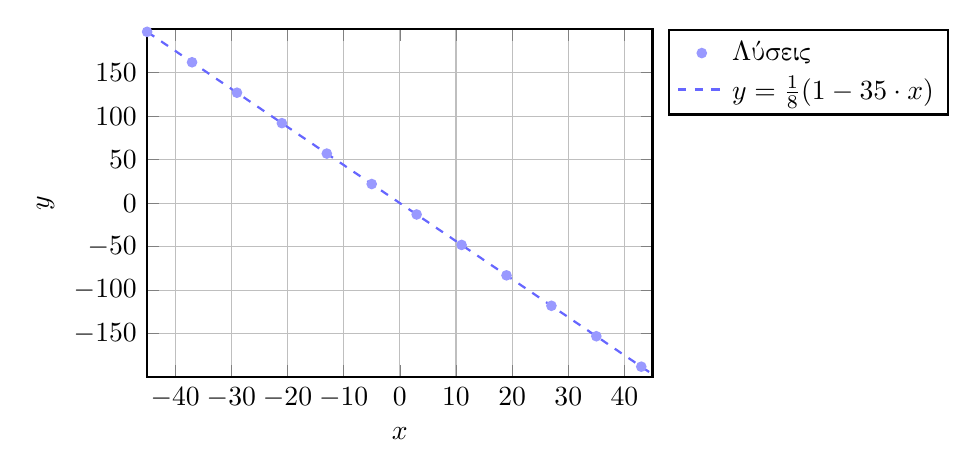
\begin{tikzpicture}
\begin{axis}[
    width=8cm,
    height=6cm,
    domain=-15:15, 
    xmin=-45,
    xmax=45,
    ymin=-200,
    ymax=200,
    thick,
    ytick={-150,-100,-50,0,50,100,150},
    xtick={-40,-30,-20,-10,0,10,20,30,40},
    legend pos=outer north east,
    mark size=1.5pt,
    xlabel={$x$},
    ylabel={$y$},
    legend cell align={left},
    grid]


\addplot[only marks, blue!40!white] coordinates {
(-45, 197)
(-37, 162)
(-29, 127)
(-21, 92)
(-13, 57)
(-5, 22)
(3, -13)
(11, -48)
(19, -83)
(27, -118)
(35, -153)
(43, -188)

};
\addlegendentry{\textgreek{Λύσεις} }

\addplot[red, domain=-50:50,restrict y to domain=-200:200, samples=100, blue!60!white,dashed]  {(1 - 35 * x) / 8 };
\addlegendentry{$y = \frac{1}{8} (1 - 35 \cdot x)$ }


\end{axis}
\end{tikzpicture}
\end{document}
